\iffalse
It's unfair to say that mathematicians aren't real doctors, we perform surgeries all the time. In this class we'll introduce the notion of a topological manifold via simplicial (delta) complexes. Spend a day or two doing examples and go over several notions like orientation, cobordism and of course surgery.

Keywords: simplicial complex, manifold, orientation, cobordism, surgery

Type: Lecture
Homework: Recommended
Prereqs: None
\fi




\documentclass{article}
\usepackage{amsmath, amsthm}
\usepackage{amssymb}
\usepackage{mathtools}
\usepackage[all,cmtip]{xy}
\usepackage{color}


\setcounter{tocdepth}{4}

\renewenvironment{proof}{ {\bfseries Proof:}}{\qed}

\newtheoremstyle{mytheorem}%                % Name
{}%                                     % Space above
{}%                                     % Space below
{\itshape}%                                     % Body font
{0pt}%\parindent}%                                     % Indent amount
{\bfseries}%                            % Theorem head font
{.}%                                    % Punctuation after theorem head
{ }%                                    % Space after theorem head, ' ', or \newline
{}%                                     % Theorem head spec (can be left empty, meaning `normal')

\theoremstyle{mytheorem}
\newtheorem{thm}{Theorem}[section]
\newtheorem{proposition}[thm]{Proposition}
\newtheorem{lemma}[thm]{Lemma}
\newtheorem{corollary}[thm]{Corollary}


\newtheoremstyle{mydefinition}%                % Name
{}%                                     % Space above
{}%                                     % Space below
{}%                                     % Body font
{0pt}%\parindent}%                                     % Indent amount
{\bfseries}%                            % Theorem head font
{.}%                                    % Punctuation after theorem head
{ }%                                    % Space after theorem head, ' ', or \newline
{}%                                     % Theorem head spec (can be left empty, meaning `normal')

\theoremstyle{mydefinition}
\newtheorem{definition}[thm]{Definition}
\newtheorem{example}[thm]{Example}
\newtheorem{exercise}[thm]{Exercise}
\newtheorem{remark}[thm]{Remark}
%\newtheorem{ques}[thm]{Q.}
\newtheorem*{ques}{Question}
%\newtheorem{ans}[thm]{Ans.}
\newtheorem*{ans}{Ans}



\numberwithin{equation}{section}

%Real numbers, complex numbers, etc.
\newcommand{\R}{\mathbb{R}}
\newcommand{\C}{\mathbb{C}}
\newcommand{\Z}{\mathbb{Z}}
\newcommand{\Q}{\mathbb{Q}}
\renewcommand{\P}{\mathbb{P}}

%How does latex not have these?
\DeclareMathOperator{\Ad}{Ad}
\DeclareMathOperator{\ad}{ad}
\DeclareMathOperator{\tr}{tr}
\DeclareMathOperator{\Tr}{Tr}
\DeclareMathOperator{\Hom}{Hom}
\DeclareMathOperator{\Spec}{Spec}
\DeclareMathOperator{\im}{im}
\DeclareMathOperator{\rank}{rank}
\DeclareMathOperator{\Exists}{\exists}
\DeclareMathOperator{\Forall}{\forall}

\DeclareMathOperator*{\colim}{colim}
\DeclareMathOperator*{\holim}{holim}
\DeclareMathOperator*{\hocolim}{hocolim}


%fractions and inner product
\newcommand{\pr}[2][\:]{\frac{\partial #1}{\partial #2}}
\newcommand{\innerp}[2]{\langle #1, #2 \rangle}

\newcommand*\conj[1]{\overline{#1}}
\newcommand*\norm[1]{\lVert #1 \rVert}

\renewcommand{\figurename}{Fig.}
\usepackage{float}
\usepackage{wrapfig}

\usepackage{enumitem}
\setlist[enumerate]{itemsep=0mm}
\usepackage{geometry}
\geometry{
	a4paper,
	total={170mm,257mm},
	left=20mm,
	top=20mm
}


\usepackage{fancyhdr}
\pagestyle{fancy}
\lhead{\scshape Apurva Nakade}
%\rhead{\scshape Mathcamp 2017}
\renewcommand*{\thepage}{\small\arabic{page}}

\rhead{\scshape Mathcamp 2017 : All things Manifoldy}

\begin{document}
\title{What is a manifold?}
\author{Apurva Nakade}
\thispagestyle{fancy}
\maketitle


\section{Introduction}
\begin{quote}
	The goal of this class is to
	\begin{enumerate}
		\item understand what manifolds are
		\item how mathematicians manipulate manifolds
		\item how to `visualize' higher dimensional manifolds
	\end{enumerate}
\end{quote}

Let us start with some motivation. One of the first objects one encounters in geometry is the plane $\R^2$.  Two nice mathematical properties that the plane has are that \begin{enumerate}
\item Every point in the plane is determined uniquely by exactly $2$ \emph{coordinates}.
\item We can measure distances between any two points on the plane.
\end{enumerate}

In everyday life we hijack these properties of the plane and use them on objects different from the plane. Consider the surface of Earth for example. Within a small area, say a city, every point can be represented by exactly 2 coordinates and we can measure the distance between any points without really worrying about the curvature of the earth.

However things get a little glitchy once we move to larger scales. We have the latitude/longitude coordinate system for all the points on the surface of the Earth but
\begin{enumerate}
	\item The assignment of longitudes is not continuous, at a few places it jumps abruptly from $-180^\circ$ to $180^{\circ}$.
	\item The poles do not posses a unique longitude.
\end{enumerate}

It also gets increasingly harder to measure distances on larger scales and it becomes necessary to take the curvature of Earth into account. (Along which line should the distance between Seattle and Berlin be measured?) These properties are what characterize a manifold. It is an object which on small scales looks very much a `Euclidean space', but this is no longer true when you zoom out.

\iffalse
One of the first examples of manifolds came from physics. When studying movements of $n$ particles subject to certain constraints the space of possible positions and momentums of these $n$ particles (also called the phase space) forms a $2n$ dimensional \textbf{symplectic manifold}. And the evolution of a system corresponds to lines in the phase space. So studying particle mechanics can be reduced to studying symplectic manifolds.

Another interesting example of a manifold comes from relativity. General relativity says that our universe is a 4 dimensional \textbf{Lorentzian manifold}, however it does not say \emph{which} Lorentzian manifold it is. So the more we know about 4 dimensional Lorentzian manifolds the better we understand our universe. String theories go further an say that perhaps our universe is in fact a much higher dimensional manifold, but perhaps we'll never know.

Manifold theory has been recently applied to big data. Consider a data set consisting of images of say, faces. Every image has thousands of pixels so the entire data set lives inside a (several) thousand dimensional vector space. Such large vector spaces are extremely difficult to analyze. Fortunately for us, many of the data sets live close to low dimensions submanifolds of these vector spaces. Manifold learning is a technique that searches for these low dimensional manifolds and leads to dimension reduction.
\fi

%%%%%%%%%%%%%%%%%%%%%%%%%%%%%%%%%%%%%%%%%%%%%%%%%%%%%%%%%%%%
%%%%%%%%%%%%%%%%%%%%%%%%%%%%%%%%%%%%%%%%%%%%%%%%%%%%%%%%%%%%
\section{Examples of manifolds}
Let us try to make the above observations more precise.

Some of the most useful objects studied in mathematics are the Euclidean spaces $\R^n$, the set of $n$ tuples of real numbers, $\R^n = \{ (x_1, \cdots, x_n) \}$. We usually think of $\R^1$ as the line, $\R^2$ as the plane, $\R^3$ as the space.
\begin{figure}[H]
	\centering 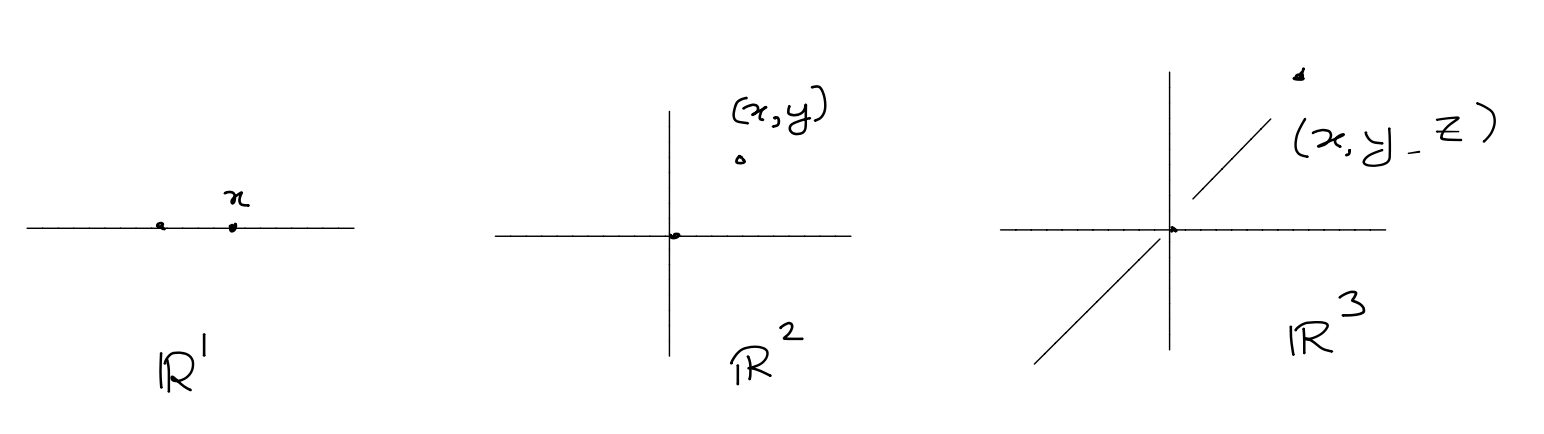
\includegraphics[width=\linewidth]{../images/EuclideanSpaces}
	\caption{Euclidean spaces}
\end{figure}

It is a useful trick in mathematics to take various properties of simple objects and study them one at a time, in the process creating other interesting objects with similar properties. For example, in the case of Euclidean space it is possible to add any two elements in $\R^n$ and get another element in $\R^n$. This generalizes to {vector spaces} and leads to {linear algebra}.

Another set of properties that Euclidean spaces have are what might be called \emph{geometric} or \emph{topological} properties.
\begin{enumerate}
	\item Every point in $\R^n$ is determined uniquely by exactly $n$ {coordinates}.
	\item It is possible to do calculus on $\R^n$.
	\item We can measure distances between points in $\R^n$.
\end{enumerate}
The objects which share these properties with Euclidean spaces are called manifolds. A \textbf{topological manifold} in an object in which every point can be \emph{locally} described by coordinates. A \textbf{smooth manifold} in an object on which it is possible to do calculus. A \textbf{Riemannian manifold} is an object on which it is possible to measure lengths of line segments.

A \textbf{manifold} is an object such that every point on it has a \emph{neighborhood} surrounding it which \emph{looks like} a Euclidean space. The exact definition of \emph{looks like} depends upon which geometric/topological property we want the manifold to have. We'll stick to the simplest kind of manifolds - topological manifolds, these are objects in which every point has a neighborhood which can be described uniquely by $n$ coordinates. The number of coordinates $\mathbf{n}$ is called the \textbf{dimension} of the manifold.

Let us see some examples and non-examples of manifolds.

\begin{example}[$S^2$]
	The surface of the Earth that we saw earlier is denoted by $S^2$, the 2 dimensional sphere
	\begin{figure}[ht]
		\centering 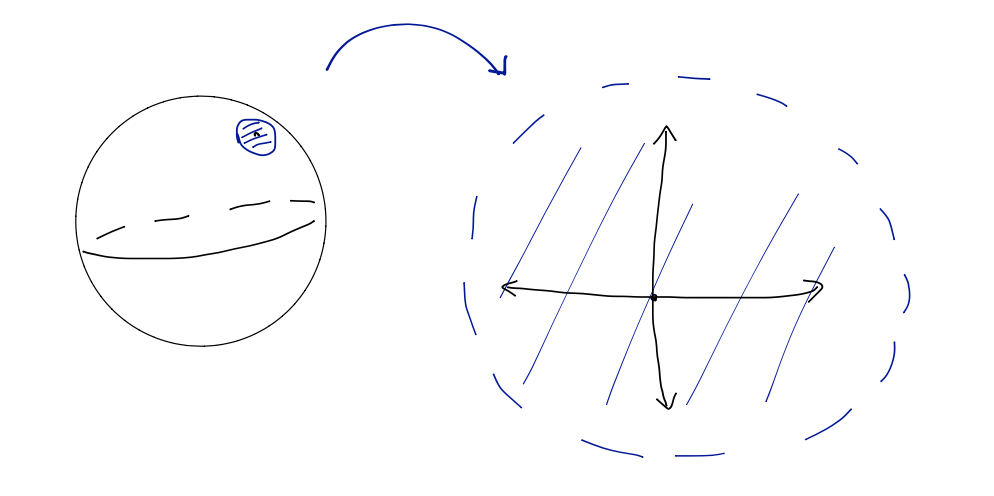
\includegraphics[width=0.8\linewidth]{../images/SphereAsAManifold}
		\caption{Every point on $S^2$ has a neighborhood that \emph{looks like} the plane $\R^2$}
	\end{figure}
\end{example}

\begin{example}[$\R^n$]
	Euclidean spaces are themselves manifolds (they better be as manifolds are modeled on them) and $\R^n$ has dimension $n$.
\end{example}

% \begin{example}[0-dimensional manifolds]
% 	Can there be 0-dimensional manifolds? Is there an $\R^0$? In a 0 dimensional manifold every point should have a neighborhood in which every point can be described by 0 coordinates, this amounts to saying that there are no other points in the neighborhood so that 0-dimensional manifolds are nothing but \textbf{isolated points}.
% 	\begin{figure}[ht]
% 		\centering \includegraphics[width=0.5\linewidth]{../images/ZeroDimManifolds}
% 		\caption{0 dimensional manifolds}
% 	\end{figure}
% \end{example}


\begin{example}[1-dimensional manifolds]
	1 dimensional manifolds are objects which locally look like lines.
	\begin{figure}[H]
		\centering 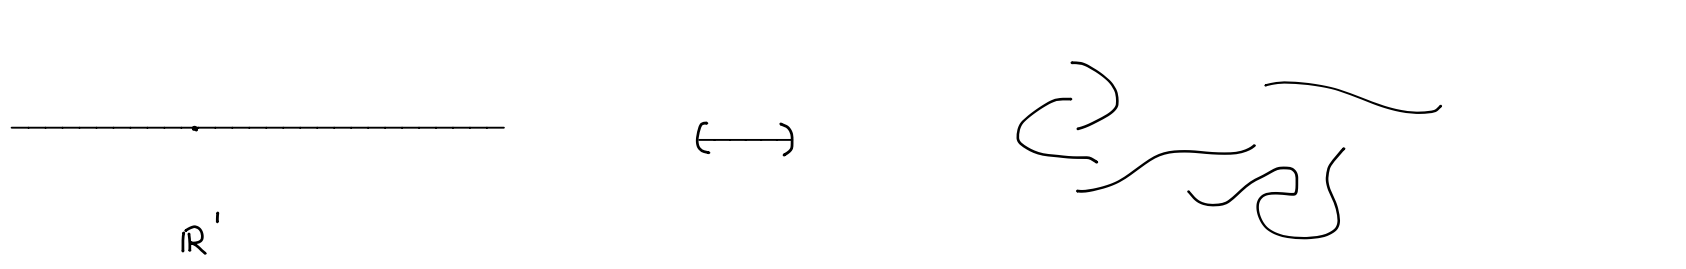
\includegraphics[width=0.75\linewidth]{../images/LineSegments}
		\caption{$\R^1$, Open internval $(a,b) \subset \R^1$ and collection of \textit{open} line segments in $\R^2$ are 1-dim manifolds}
	\end{figure}
	\begin{figure}[H]
		\centering 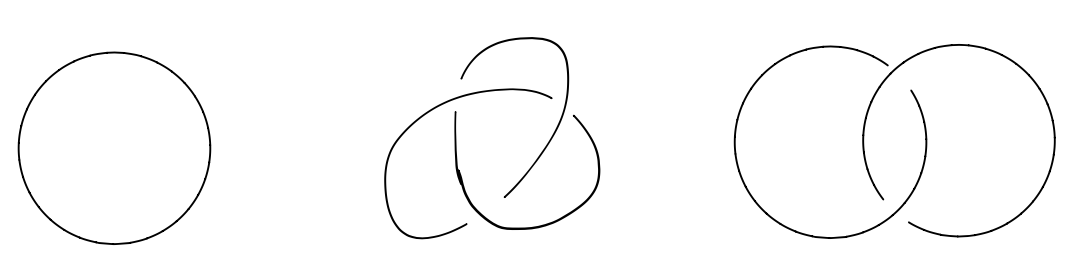
\includegraphics[width=0.75\linewidth]{../images/Knots}
		\caption{Circle, trefoil and Hopf link are 1-dim manifolds}
	\end{figure}

	The following examples are NOT manifolds. The union of $x$ and $y$ axes is not a manifold as no neighborhood of the origin $(0,0)$ \emph{looks like} a Euclidean space. The space of non-negative real numbers is not a manifold because the point $0$ does not have a neighborhood which looks like a Euclidean space (it only \emph{looks like} half the Euclidean space $\R^1$), same argument holds for non-open intervals $[a,b]$ or $[a,b)$.
		\begin{figure}[H]
			\centering 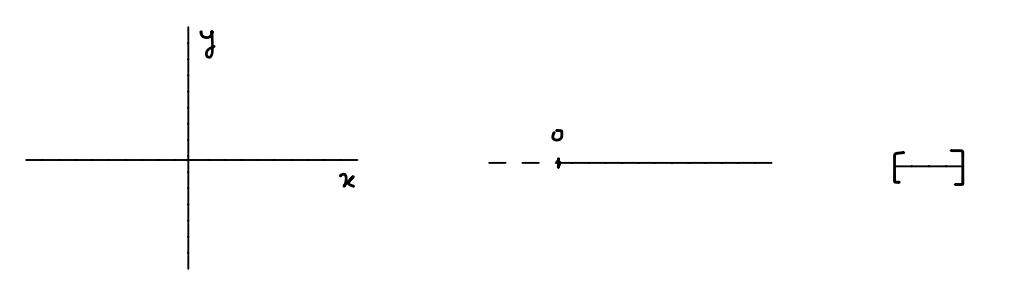
\includegraphics[width=0.75\linewidth]{../images/NonExamplesOfManifolds}
			\caption{Union of $x$ and $y$ axes in $\R^2$, the space of non-negative real numbers, closed interval $[a,b]$ are not manifolds}
		\end{figure}
	\end{example}



	\begin{example}[Surfaces]
		The surface of a donut is called a \textbf{torus}. Because it has 1 `hole' in it the torus is also called a \textbf{genus 1} surface. More generally surfaces with $g$ holes are called genus $g$ surfaces.
		\begin{figure}[H]
			\centering 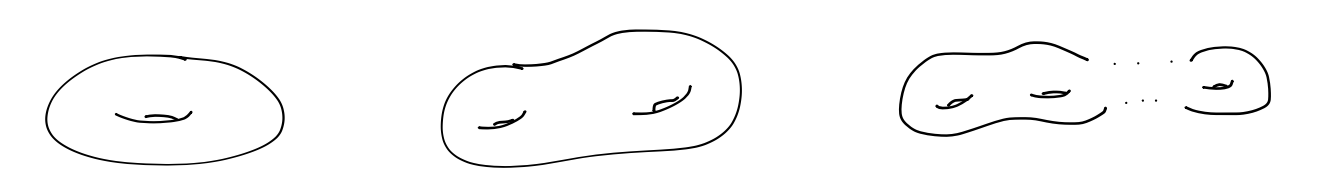
\includegraphics[width=0.85\linewidth]{../images/GegusGSurfaces}
			\caption{Torus, genus 2 surface, higher genus surfaces}
		\end{figure}
		We can remove points from a torus to get a punctured torus. Such manifolds are very interesting mathematically and are extensively studied in hyperbolic geometry.
		\begin{figure}[H]
			\centering 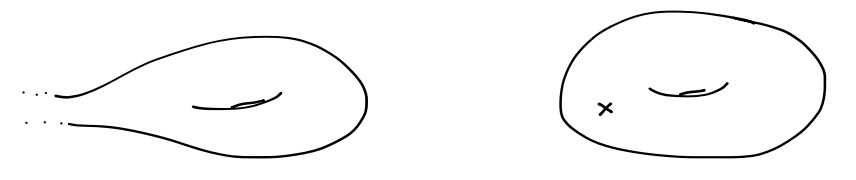
\includegraphics[width=0.55\linewidth]{../images/PuncturedTorus}
			\caption{Torus with an end and a punctured torus}
		\end{figure}
	\end{example}

	\begin{example}[Spheres]
		The set $S^{n-1} \subset \R^n$ is defined as
		\begin{align*}
			S^{n-1} = \{ (x_1, \cdots, x_n) : x_1^2 + x_2 ^{2} + \cdots x_n ^{2} = 1 \}
		\end{align*}
		This is the $n-1$ dimensional \textbf{sphere} (and a manifold) sitting inside $\R^n$.
	\end{example}



	% \begin{example}
	% 	The set of rotations (and also translations) of $\R^n$ is a manifold. When $n=2$ this is the space of rotations of $\R^2$ but this space is just the circle and hence a manifold!
	%
	% 	When $n=3$ the manifold is difficult to imagine. In this case the coordinates are given by what are called \textbf{Euler angles}.
	% \end{example}








	%%%%%%%%%%%%%%%%%%%%%%%%%%%%%%%%%%%%%%%%%%%%%%%%%%%%%%%%%%%%
	%%%%%%%%%%%%%%%%%%%%%%%%%%%%%%%%%%%%%%%%%%%%%%%%%%%%%%%%%%%%
	\section{Definition of a manifold}
	To define `looks like' we need the concept of \textbf{continuity} from point set topology. A continuous map is a map which does not break things apart, another way of saying the same thing is that nearby points go to nearby points. Let us make this more precise.

	Let $A, B$ be subsets of $\R^n$ where $n$ is a positive integer.

	\begin{definition}
		A sequence of points $x_1, x _ 2, \cdots , x_i, \cdots \in A$ is said to converge to a point $x \in A$, denoted $x_i \rightarrow x$, if the distance between $x_i$ and $x$ goes to 0 as $i \rightarrow \infty$.
		\begin{align}
			\lim \limits _ {i \rightarrow \infty} \norm{x - x_i} = 0 & \implies x_i \rightarrow x
		\end{align}
	\end{definition}

	\begin{definition}
		A map $f: A \rightarrow B$ is said to be \textbf{continuous at} $\mathbf{a} \in A$ if for every sequence $x_i \rightarrow a$ in $A$ the sequence $f(x_i) \rightarrow f(a)$ in $B$. If $f: A \rightarrow B$ is continuous at every point $a \in A$ then $f$ is called a \textbf{continuous map}.
	\end{definition}

	We're now ready to define `looks like':
	\begin{definition}
		We say $A$ and $B$ are homeomorphic if there exist \emph{continuous} maps $f: A \rightarrow B$ and $g: B \rightarrow A$ such that for all points $a\in A$ and $b \in B$ we have $f(g(b)) = b$ and $g(f(a)) = a$.
	\end{definition}
	This then is going to be our version of `looks like'.

	\begin{definition}[Topological manifold]
		A set $M \subseteq \R^n$ is called a topological manifold if for each point $a$ in $A$ there exists an open subset $U$ containing $a$, called a \textbf{neighborhood} of $a$, such that $U$ is homeomorphic to $\R^k$ for some $k$.
	\end{definition}

	To be precise the definition above is that of a \textbf{submanifold} of ${\R^n}$. We can allow $M$ to be a topological space (with some technical restrictions) devoid of any ambient $\R^n$.

	For the purposes of this class we'll think of two homeomorphic manifolds as being the same manifold. It is not hard to see that if one manifold can be continuously deformed into another then the two manifolds are homeomorphic. This gives rise to the infamous for-a-topologist-cup-is-the-same-as-a-donut joke.

	\begin{figure}[H]
		\centering
		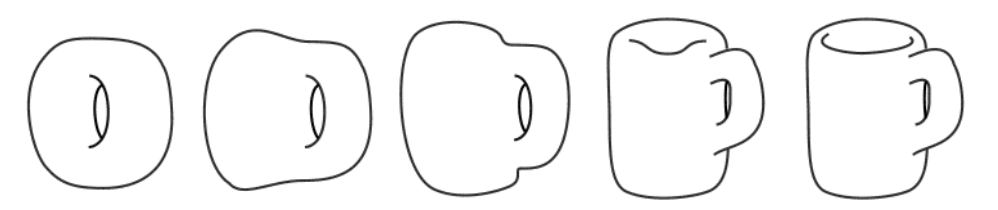
\includegraphics[width=0.75\linewidth]{../images/Torus-Mug}
		\caption{A cup is diffeomorphic to a donut}
	\end{figure}




	\section{Exercises}

	\begin{exercise}
		Use the above deformation diagram to explicitly `construct' a homeomorphism between a torus and teacup.
	\end{exercise}

	\begin{exercise}
		Show that homeomorphism is an equivalence relation.
	\end{exercise}

	\begin{exercise}
		Show that any two open intervals $(a,b)$ and $(c,d)$ are homeomorphic.
	\end{exercise}

	\begin{exercise}
		Prove that $[0,1]$ is not a manifold.
	\end{exercise}


	\begin{exercise}
		Use the following exercise to explicitly prove that $S^{n-1}$ is a manifold of $\dim n-1$.
		\begin{enumerate}
			\item Consider the set $S^1 = \{ (x_1,x_2) : x_1^2 + x_2^2 = 1\}$. Let $N = (0,1) \in S^1$ be the `north pole'. Explicitly describe the \emph{stereographic projection} map from the north pole
			      \begin{figure}[H]
			      	\centering
			      	
\includegraphics[width=0.25\linewidth]{../images/StereoProj}
			      	\caption{$f:S^1 \setminus \{n\} \rightarrow \R^2$, $P \mapsto P'$}
			      \end{figure}
			\item Repeat the same for $S^2$ and generalize to $S^{n-1}$.
		\end{enumerate}
	\end{exercise}

	% \begin{exercise}
	% 	What is the largest neighborhood of a point in $S^1$ and $S^2$ which looks like $\R^1$ and $\R^2$ respectively?
	% \end{exercise}
	%
	% \begin{exercise}\label{thm:polynomialExercise}
	% 	\begin{enumerate}
	% 		\item Draw the set of points in $\R^2$ which satisfy each of the following equations:\\
	% 		      i) $x^2 + y^2 = 1$ ii) $xy = 0$ iii) $y^2 - x^2(x+1) = 0$. Which of these sets are manifolds?
	% 	\end{enumerate}
	% \end{exercise}



	\subsection{Obstructions}
	To show that two sets are homeomorphic or to show that a space is a manifold we need to construct appropriate maps. But showing two spaces are {NOT} homeomorphic or that a space is {NOT} a manifold requires a completely different proof.

	In topology such proof techniques fall under the umbrella of \textbf{obstruction theory}. The simplest obstruction is the size of a set, a finite set cannot be homeomorphic to an infinite one and two finite sets of different sizes cannot be homeomorphic to each other.

	The next obstruction is connectedness.

	\begin{exercise}
		A set $A \subset \R^n$ is called (path)connected if any two points in $A$ can be connected by a path lying entirely in $A$.
		\begin{enumerate}
			\item Show that if $A$ is connected and $A$ is homeomorphic to $B$ then $B$ is also connected.
			\item Show that no two of the spaces $(0,1)$, $[1,0]$ and $S^1$ are homeomorphic to each other.
			\item Show that $\R^1$ is not homeomorphic to $\R^2$.
			\item Show that a 1 dimensional manifold is not homeomorphic to a 2 dimensional manifold.
		\end{enumerate}
	\end{exercise}
	The set of connected components of $A$ is denoted by $\pi_0(A)$. By the above exercise $A$ is homeomorphic to $B$ only if $\pi_0(A) \cong \pi_0(B)$. Hence we say that $\pi_0$ is a topological invariant. $\pi_0$ is a very useful invariant when trying to distinguish 1 dimensional manifolds but is quite weak for higher dimensional ones.

	To be able to distinguish higher dimensional manifolds topologists have created several invariants like higher homotopy groups $\pi_1, \pi_2, \cdots$,  homology groups $H_0, H_1, \cdots$,  cohomology groups $H^0, H^1, \cdots$, generalized (co)homology theories $E_*$, $E^*$ which provide stronger obstructions to existence of homeomorphisms.\\

	Try the following exercise which is beyond the scope of this class and needs the next obstruction $\pi_1$ or $H_1$.
	\begin{exercise}
		Is the torus homeomorphic to the sphere $S^2$? Is $\R^2$ homeomorphic to $\R^3$?
	\end{exercise}

\end{document}
